\begin{alist}
\item Η συνάρτηση $\varphi$ έχει πεδίο ορισμού το $\mathbb{R}$, επομένως για κάθε $x \in \mathbb{R}$ το $-x \in \mathbb{R}$.
Επιπλέον για κάθε $x \in \mathbb{R}$ ισχύει: $\varphi(-x) = 3(-x)^2 = 3x^2 = \varphi(x)$.
Επομένως είναι άρτια συνάρτηση.

Η γραφική της παράσταση είναι η παρακάτω παραβολή.

\begin{center}
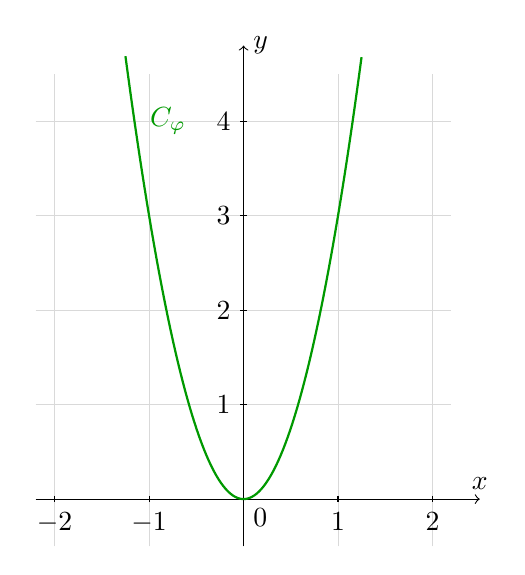
\begin{tikzpicture}[x=1cm,y=1cm,scale=1.2]
\draw[step=1cm,gray!30,very thin] (-2.2,-0.5) grid (2.2,4.5);
\draw[->] (-2.2,0) -- (2.5,0) node[above] {$x$};
\draw[->] (0,-0.5) -- (0,4.8) node[right] {$y$};
\foreach \x in {-2,-1,1,2} \draw (\x cm,1pt) -- (\x cm,-1pt) node[anchor=north] {$\x$};
\foreach \y in {1,2,3,4} \draw (1pt,\y cm) -- (-1pt,\y cm) node[anchor=east] {$\y$};
\node[below right] at (0,0) {$0$};

\draw[green!60!black, thick, domain=-1.25:1.25, samples=100] plot (\x,{3*\x*\x});
\node[green!60!black] at (-0.8, 4) {$C_\varphi$};
\end{tikzpicture}
\end{center}

\item Είναι:
\[f(x) = 3x^2 - 6x + 8 = 3\left(x^2 - 2x + \dfrac{8}{3}\right) = 3\left(x^2 - 2x + 1 + \dfrac{5}{3}\right) = 3\left[(x - 1)^2 + \dfrac{5}{3}\right]\]
Επομένως $f(x) = 3(x - 1)^2 + 5$, $x \in \mathbb{R}$.

Η γραφική παράσταση της $f$ προκύπτει από δύο διαδοχικές μετατοπίσεις της γραφικής παράστασης της $\varphi$, μιας οριζόντιας κατά 1 μονάδα προς τα δεξιά και μιας κατακόρυφης κατά 5 μονάδες προς τα πάνω. Έτσι, είναι:
\end{alist}
